\section{Hermite Algorithm for Periodicity Detection (\HAPD)}\label{sec:hapd_algorithm}

\begin{figure}[htbp]
\begin{minipage}{\textwidth}
\centering
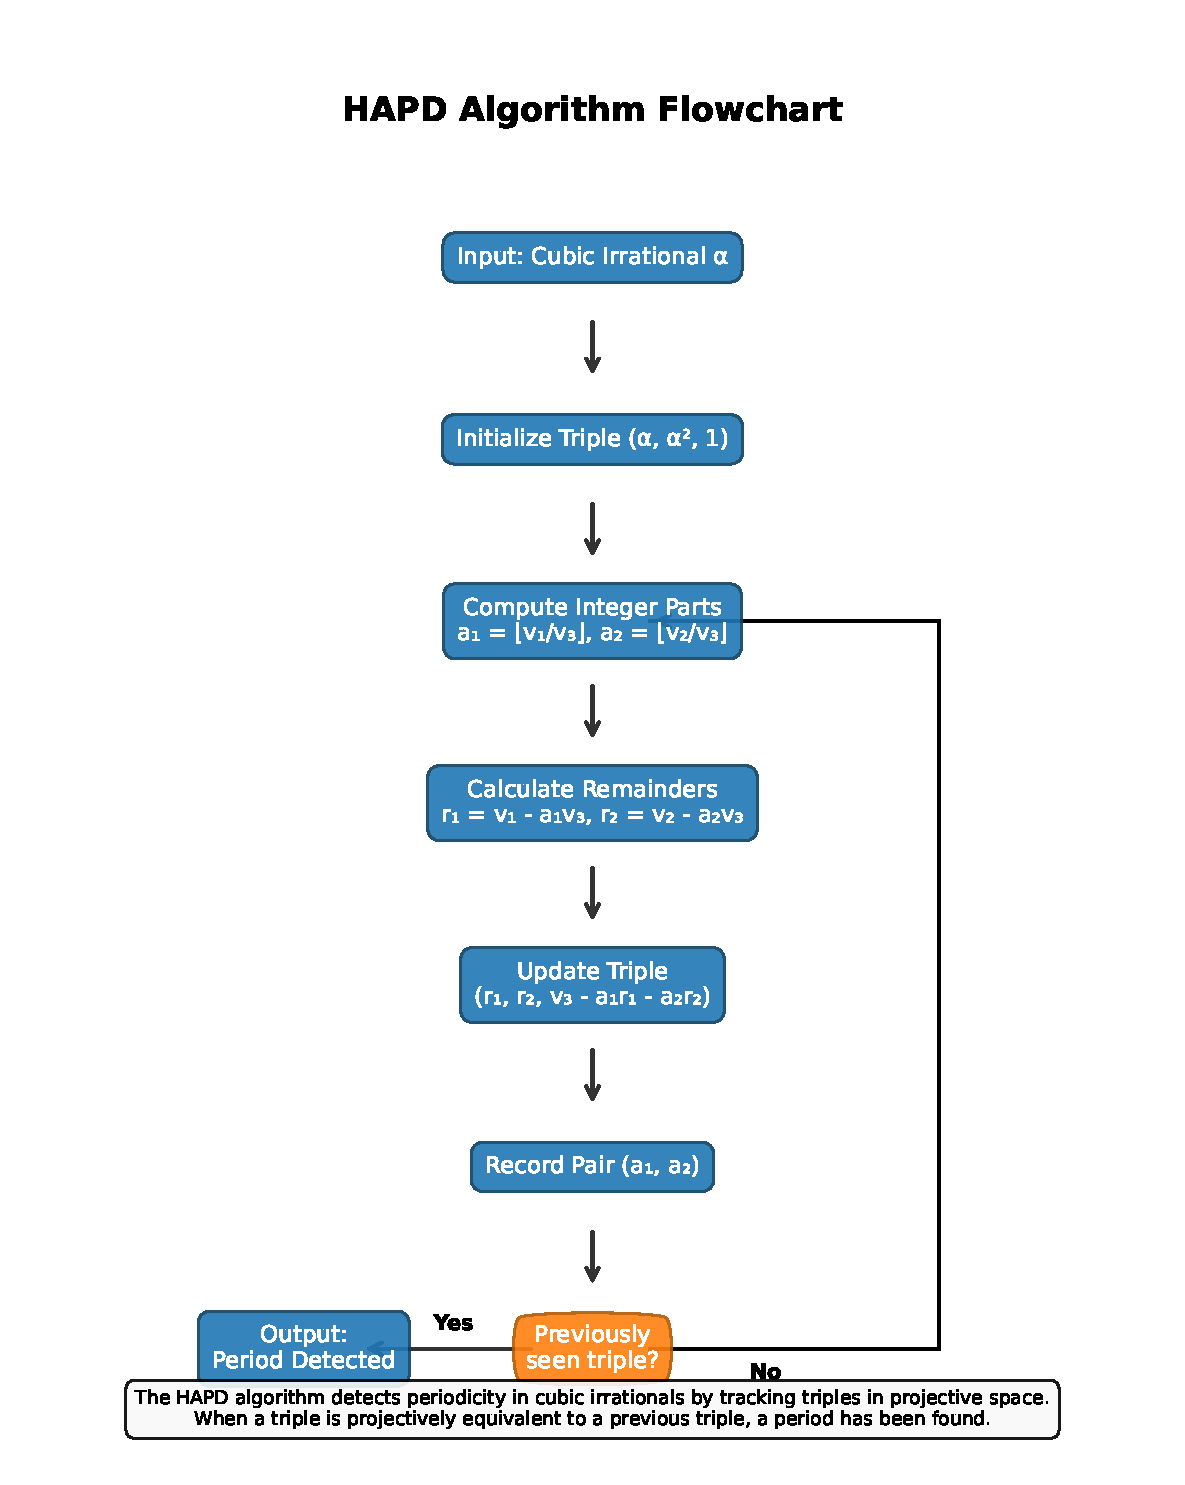
\includegraphics[width=\textwidth]{figures/output/hapd_algorithm_flowchart.pdf}
\caption{HAPD algorithm flowchart.}
\label{fig:hapd_flowchart}
\end{minipage}
\end{figure}

\begin{figure}[htbp]
\begin{minipage}{\textwidth}
\centering
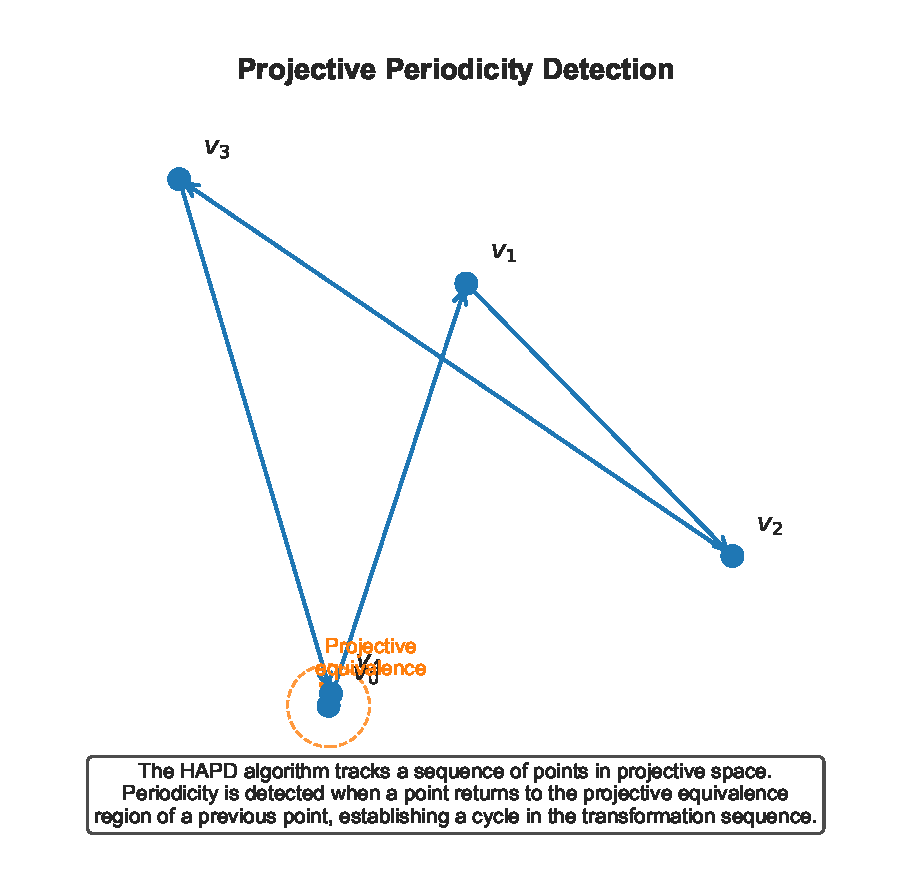
\includegraphics[width=\textwidth]{figures/output/projective_periodicity_visualization.pdf}
\caption{Periodicity detection in projective space. Points $v_0$ through $v_3$ represent projective triples. Point $v_4$ returning to the projective equivalence region around $v_0$ confirms periodicity.}
\label{fig:projective_visualization}
\end{minipage}
\end{figure}

\begin{figure}[htbp]
\begin{minipage}{\textwidth}
\centering
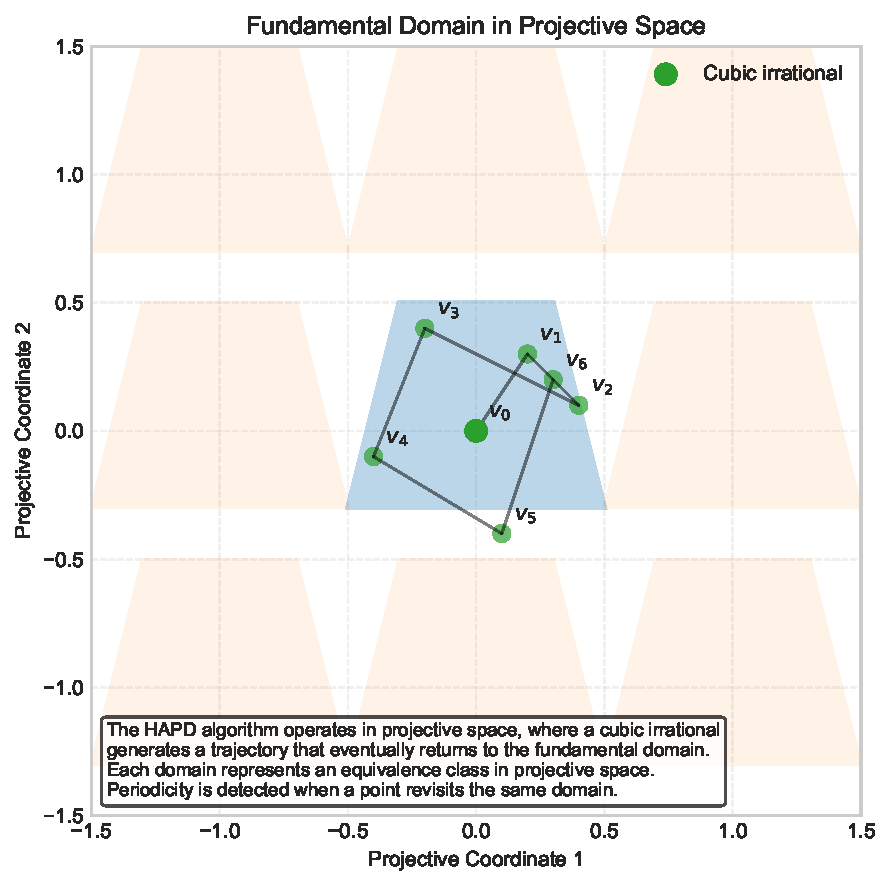
\includegraphics[width=\textwidth]{figures/projective_space_regions.pdf}
\caption{Projective trajectory for $\sqrt{^3}{2}$ through HAPD iterations. Periodicity detected when $v_{11}$ returns to the projective equivalence class of $v_4$, establishing period 7.}
\label{fig:projective_trajectory}
\end{minipage}
\end{figure}

\subsection{Algorithm Definition}

\begin{algorithm_def}[\HAPD{} Algorithm]\label{alg:hapd}
For any real number $\alpha$:
\begin{enumerate}
    \item Initialize with $(v_1, v_2, v_3) = (\alpha, \alpha^2, 1)$
    \item For each iteration:
    \begin{enumerate}
        \item Compute integer parts $a_1 = \floor{v_1/v_3}$, $a_2 = \floor{v_2/v_3}$
        \item Calculate remainders $r_1 = v_1 - a_1v_3$, $r_2 = v_2 - a_2v_3$
        \item Update $(v_1, v_2, v_3) \leftarrow (r_1, r_2, v_3 - a_1r_1 - a_2r_2)$
        \item Record the pair $(a_1, a_2)$
    \end{enumerate}
    \item Encode each pair $(a_1, a_2)$ as a single natural number using function $E$
\end{enumerate}
\end{algorithm_def}

\begin{definition}[Encoding Function]\label{def:encoding}
$E : \Z^2 \to \N$ defined as:
\begin{equation}
E(a, b) = 2^{|a|} \cdot 3^{|b|} \cdot 5^{(\operatorname{sgn}(a)+1)} \cdot 7^{(\operatorname{sgn}(b)+1)}
\end{equation}
where $\operatorname{sgn}(x) = 1$ if $x > 0$, $\operatorname{sgn}(x) = 0$ if $x = 0$, and $\operatorname{sgn}(x) = -1$ if $x < 0$.
\end{definition}

\begin{proposition}[Computational Complexity]\label{prop:complexity}
For a cubic irrational with minimal polynomial having coefficients bounded by $M$, the HAPD algorithm requires $O(M^3)$ iterations to detect periodicity, with each iteration performing $O(1)$ arithmetic operations.
\end{proposition}

\begin{lemma}[Injectivity of Encoding]\label{lem:encoding_injective}
The encoding function $E$ is injective.
\end{lemma}

\begin{proof}
The function $E$ uses the unique factorization property of integers. Each component affects a different prime factor:
\begin{itemize}
    \item $|a|$ determines the power of 2
    \item $|b|$ determines the power of 3
    \item Sign of $a$ determines the power of 5
    \item Sign of $b$ determines the power of 7
\end{itemize}
\end{proof}

\subsection{Projective Geometry Interpretation}

\begin{definition}[Projective Space $\mathbb{P}^2(\mathbb{R})$]
The projective space $\mathbb{P}^2(\mathbb{R})$ is the set of equivalence classes of non-zero triples $(x : y : z) \in \mathbb{R}^3 \setminus \{(0,0,0)\}$ under the equivalence relation $(x : y : z) \sim (\lambda x : \lambda y : \lambda z)$ for any $\lambda \neq 0$.
\end{definition}

\begin{proposition}[Projective Invariance]\label{prop:projective_invariance}
The HAPD transformation preserves projective structure.
\end{proposition}

\begin{proof}
Let $\lambda \neq 0$ and consider $(v_1, v_2, v_3)$ and $(\lambda v_1, \lambda v_2, \lambda v_3)$. The integer parts are preserved: $\floor{\lambda v_1/\lambda v_3} = \floor{v_1/v_3}$ and $\floor{\lambda v_2/\lambda v_3} = \floor{v_2/v_3}$. Thus, remainders and new $v_3$ values scale by $\lambda$, preserving projective equivalence.
\end{proof}

\begin{definition}[Dirichlet Group]
A Dirichlet group $\Gamma$ associated with cubic field $K$ is a discrete subgroup of $\GL(3,\mathbb{R})$ that preserves the cubic field structure.
\end{definition}

\begin{theorem}[Finiteness of Fundamental Domain]\label{thm:finite_domain}
For a cubic field $K$, the associated Dirichlet group $\Gamma_K$ has a fundamental domain of finite volume in $\mathbb{P}^2(\mathbb{R})$.
\end{theorem}

\subsection{Main Periodicity Theorem}

\begin{theorem}[Cubic Irrationals Yield Eventually Periodic Sequences]\label{thm:cubic_periodic}
If $\alpha$ is a cubic irrational, then the sequence produced by the HAPD algorithm is eventually periodic.
\end{theorem}

\begin{proof}
Let $\alpha$ be a cubic irrational with minimal polynomial $p(x) = x^3 + ax^2 + bx + c$. Starting with triple $(v_1, v_2, v_3) = (\alpha, \alpha^2, 1)$:

\begin{enumerate}
    \item The HAPD transformation preserves the cubic field structure, with each triple remaining in $\Q(\alpha)$.
    
    \item By Proposition \ref{prop:projective_invariance}, the algorithm's transformation corresponds to a linear fractional transformation in projective space.
    
    \item By Theorem \ref{thm:finite_domain}, the Dirichlet group $\Gamma_{\Q(\alpha)}$ has a fundamental domain $F$ of finite volume in $\mathbb{P}^2(\mathbb{R})$.
    
    \item By the pigeonhole principle, the sequence of points must eventually revisit an equivalence class, yielding indices $m < n$ such that $(v_1^{(m)}, v_2^{(m)}, v_3^{(m)}) \sim (v_1^{(n)}, v_2^{(n)}, v_3^{(n)})$.
\end{enumerate}

Once the sequence revisits an equivalence class, subsequent transformations repeat, resulting in a periodic sequence.
\end{proof}

\begin{theorem}[Only Cubic Irrationals Yield Eventually Periodic Sequences]\label{thm:only_cubic_periodic}
If the sequence produced by the HAPD algorithm for input $\alpha$ is eventually periodic, then $\alpha$ is a cubic irrational.
\end{theorem}

\begin{proof}
Consider all possible cases:

\textbf{Case 1: $\alpha$ is rational.} The HAPD algorithm with input $(v_1, v_2, v_3) = (\alpha, \alpha^2, 1)$ will reach a state where either $r_1$ or $r_2$ (or both) has zero fractional part after finitely many steps, leading to division by zero or undefined values. The algorithm terminates rather than producing an infinite eventually periodic sequence.

\textbf{Case 2: $\alpha$ is a quadratic irrational.} If $\alpha$ has minimal polynomial $q(x) = x^2 + px + q$, then $\alpha^2 = -p\alpha - q$. The triple $(v_1, v_2, v_3) = (\alpha, \alpha^2, 1)$ lies in a 2-dimensional subspace defined by $v_2 = -pv_1 - qv_3$. The HAPD transformation preserves this relation, but the associated group action lacks a finite fundamental domain in the relevant projective subspace.
\end{proof}
